This menu provides functions of computing and visualizing influence according to a simple model described in appendence ~\ref{FadeModel}). Some of these function needs parameters which are memeorized

\subsection{Preselect Sources and Targets}
\textbf{Plugins$\Rightarrow$BiNoM$\Rightarrow$BiNoM Analysis$\Rightarrow$Fading Signal Propagation Model$\Rightarrow$Preselect Sources and Targets}\\
Preselect in dialogs nodes as sources or as targets. So, these nodes are selected, when opening list boxes, The node attribute PRESELECTED is set to 1 if source, to 2 if target, to 3 if both target and source. Not preselected node attribute is set to 0. It can be directly imported as node attribute by Cytoscape.

\subsection{Select Sub-network from Sources to Targets}
\textbf{Plugins$\Rightarrow$BiNoM$\Rightarrow$BiNoM Analysis$\Rightarrow$Fading Signal Propagation Model$\Rightarrow$Select Sub-Network From Sources to Targets}\\
This function selects nodes and edges in the network between a list of sources and a list of targets.  Loops are included in the selection. For all nodes as sources or targets: select the first node and type shift+control+end.

\subsection{Select Mono or Multi Path Mode}
\textbf{Plugins$\Rightarrow$BiNoM$\Rightarrow$BiNoM Analysis$\Rightarrow$Fading Signal Propagation Model$\Rightarrow$Select Mono or Multi Path Mode}\\
This function selects the type of exploring mode: multi path or mono path (see Appendices ~\ref{FadeModel}).

\subsection{Display Signed Distances}
\textbf{Plugins$\Rightarrow$BiNoM$\Rightarrow$BiNoM Analysis$\Rightarrow$Fading Signal Propagation Model$\Rightarrow$Display Signed Distances}\\
After selecting sources and targets, display the number of paths from sources to targets signed by weights according to the path mode (reach is only necessary for muti path mode).

\subsection{Update Influence Attribute}
\textbf{Plugins$\Rightarrow$BiNoM$\Rightarrow$BiNoM Analysis$\Rightarrow$Fading Signal Propagation Model$\Rightarrow$Update Weigth Influence Attribute}\\
A weight of influence as edge attribute must be affected to every edge. This dialog updates the weight attribute by 
\begin{itemize}
\item selecting the attribute containing the edge influence,
\item affecting its values to activation (weight=+1) and inhibition (weight=-1).
\end{itemize}
3 possible values for the attribute. Generally, the attribute is "interaction" and the values "activation" or "inhibition". Be careful of lower-case and upper-case (see~\ref{Weight_Attribute_Dialog}).

% change graphics 
\begin{figure}
\centering
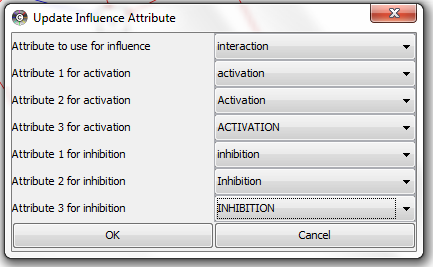
\includegraphics[width=0.7\textwidth]{graphics/Weight_Attribute_Dialog}
\caption{Dialog updating weight attribute from an other attribute}
\label{Weight_Attribute_Dialog}
\end{figure}

\subsection{Input Reach Parameter}
\textbf{Plugins$\Rightarrow$BiNoM$\Rightarrow$BiNoM Analysis$\Rightarrow$Fading Signal Propagation Model$\Rightarrow$Input Reach Parameter}\\
Input the number of paths beyond which the influence is insignificant, less than 5\%. It is a floating point number, not necessary integer.

\subsection{Display Network and Parameter Features}
\textbf{Plugins$\Rightarrow$BiNoM$\Rightarrow$BiNoM Analysis$\Rightarrow$Fading Signal Propagation Model$\Rightarrow$Display Network and Parameter Features}\\
Display in a text box: network, size of network, reach parameter, min, max, mean and standard deviation influence, computed by excluding not connected nodes. It a recapitulation of parameters and their effect on influence matrix.

\subsection{List Opened Edges MultiPath Only}
\textbf{Plugins$\Rightarrow$BiNoM$\Rightarrow$BiNoM Analysis$\Rightarrow$Fading Signal Propagation Model$\Rightarrow$List Opened Edges MultiPath Only}\\
Only in multi path mode. List edges which are opened to avoid loop and allow multi path computing.

\subsection{Display Influence Array As Text}
\textbf{Plugins$\Rightarrow$BiNoM$\Rightarrow$BiNoM Analysis$\Rightarrow$Fading Signal Propagation Model$\Rightarrow$Display Influence Array As Text}\\
The influence matrix is displayed in a text box which can be copied in the clipboard and paste in a spreadsheet, sources in columns, targets in rows, names in alphabetical order. Parameters and option are in window title.\\\\
Text window with 2 options: 
\begin{itemize}
\item for visualizing, "nc" = not connected, only 3 digits after point for numbers,
\item for computing,  all values are numeric with all possible digits,
\end{itemize}
Same dialog as "Select Sub-network from Sources to Targets".  Preselected sources and targets can be used.  For all nodes as sources or targets: select the first node and type shift+control+end.

\subsection{Display Influence As List}
\textbf{Plugins$\Rightarrow$BiNoM$\Rightarrow$BiNoM Analysis$\Rightarrow$Fading Signal Propagation Model$\Rightarrow$Display Influence As List}\\
Same result than Display Influence Array As Text For Computing, but as a list between every both nodes.


\subsection{Display Influence Array as Paved Window}
\textbf{Plugins$\Rightarrow$BiNoM$\Rightarrow$BiNoM Analysis$\Rightarrow$Fading Signal Propagation Model$\Rightarrow$Display Influence Array as Paved Window}\\
Same computing as "Display Influence Array As Text". Results are in:
\begin{itemize}
\item paved window with 2 options: 
\begin{itemize}
\item activated in red, inhibited in green, light to dark according to the value, not connected in black,
\item activated in red, inhibited in blue, light to dark according to the value, not connected in white (see~\ref{paved_window}),
\end{itemize}
\item text window where are displayed details of selected area in paved window.
\end{itemize}

\begin{figure}
\centering
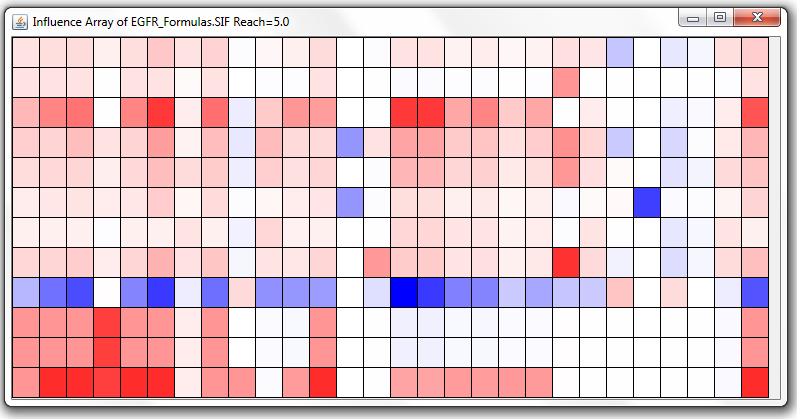
\includegraphics[width=1.0\textwidth]{graphics/paved_window}
\caption{Window paved by the level of influence between species}
\label{paved_window}
\end{figure}

\subsection{Influence by Active Nodes as Attribute}
\textbf{Plugins$\Rightarrow$BiNoM$\Rightarrow$BiNoM Analysis$\Rightarrow$Fading Signal Propagation Model$\Rightarrow$Influence by Active Nodes as Attribute}\\
Activity levels of nodes are input in an attribute "ACTIV\_IN". The result of the multiplication of influence matrix by activity level input is "ACTIV\_OUT" attribute.

\subsection{Display Influence Array Between Modules}
\textbf{Plugins$\Rightarrow$BiNoM$\Rightarrow$BiNoM Analysis$\Rightarrow$Fading Signal Propagation$\Rightarrow$Display Influence Array Between Modules}\\
Display influence array for computing, sources and targets being all nodes or modules. The influence between modules is the sum of influence of nodes inside modules. Where there is no module, the result is the same get by Display Influence Array As Text For Computing between all nodes.

\subsection{Display Influence Reach Area in Array}
\textbf{Plugins$\Rightarrow$BiNoM$\Rightarrow$BiNoM Analysis$\Rightarrow$Fading Signal Propagation Model$\Rightarrow$Display Influence Reach Area in Array}\\
Computing as "Display Influence Array for Computing" with all weights=1. Useful to appreciate the absolute level of influence by a specie to other species.

\subsection{Influence Reach Area as Attribute}
\textbf{Plugins$\Rightarrow$BiNoM$\Rightarrow$BiNoM Analysis$\Rightarrow$Fading Signal Propagation Model$\Rightarrow$Influence Reach Area as Attribut}\\
Computing from selected nodes with all weights=1. Absolute influence levels are put in attribute "INFLUENCE\_AREA\_N" where N keeps every successive results. Start nodes and options must be noted manually. Useful to visualize the influence of a group of species.

\subsection{Input Score Threshold}
\textbf{Plugins$\Rightarrow$BiNoM$\Rightarrow$BiNoM Analysis$\Rightarrow$Fading Signal Propagation Model$\Rightarrow$Input Score Threshold}\\
Input the threshold used to compute the score. 

\subsection{Compute Score of Data Sets }
\textbf{Plugins$\Rightarrow$BiNoM$\Rightarrow$BiNoM Analysis$\Rightarrow$Fading Signal Propagation Model$\Rightarrow$Compute Score of Data Sets}\\
Data must be input as node attributes:
\begin{itemize}
\item Activity levels of source nodes as input, attribute "INPUT\_\_SETidentifier" (2 underscores), identifier may be a number or a word, 
\item Expected activity levels of target nodes as output aim, attribute "OUTPUT\_AIMidentifier", identifier matches input with output.
\end{itemize}
The result is a tabulated text including size of data sets, number of maching output (with threshold) and Cohen's kappa coefficient (see~\ref{Score_Of_Data_Sets} and, about definition see~\ref{FadeModel}).
If level \textless -threshold, node is taken as inhibited. If level \textgreater +theshold, node is taken as activated.

\begin{figure}
\centering
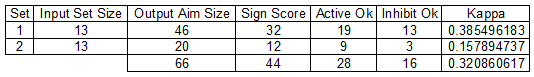
\includegraphics[width=1.0\textwidth]{graphics/Score_Of_Data_Sets}
\caption{Score of data sets formatted in a spreadsheet}
\label{Score_Of_Data_Sets}
\end{figure}

\subsection{Test Score by Reversing Sign Weight }
\textbf{Plugins$\Rightarrow$BiNoM$\Rightarrow$BiNoM Analysis$\Rightarrow$Fading Signal Propagation Model$\Rightarrow$Test Score by Reversing Sign Weights}\\
Test if reversing sign weight of every edge improves kappa, display list of egdes sorted by decreasing kappa.

\subsection{Test Score by Canceling Weight }
\textbf{Plugins$\Rightarrow$BiNoM$\Rightarrow$BiNoM Analysis$\Rightarrow$Fading Signal Propagation Model$\Rightarrow$Test Score by Cancelling Weight}\\
Test if cancelling sign weight of every edge improves kappa, display list of egdes sorted by decreasing kappa. No change in structure network.